\section{Maticové hry}
Maticová hra je \hyperref[konecna]{konečná} hra dvou hráčů s nulovým součtem.

Ať $G = (S_1, S_2, u)$ je maticová hra, kde $S_1 = \bc{\sigma_1, \dots, \sigma_m}$, $S_2 = \bc{\tau_1, \dots, \tau_n}$
a $u : S_1 \times S_2 \rightarrow \R$.

\begin{itemize}
    \item Jednoznačná korespondence mezi $u$ a maticí $A = (a_{ij}) \in \M_{m,n}(\R)$, kde 
    $a_{ij} = u(\sigma_i, \tau_j)$.
    \item $A$ $\dots$ matice hry (výplatní matice, matice úžitku, \dots)
    \item \hyperref[smisRoz]{Smíšené rozšíření} hry $G$ je hra $\Gamma(A) = (X, Y, U)$, kde
    \begin{itemize}
        \item $X = \bc{x \in \R_+^m \middle| \sum_{i=1}^{m} x_i=1}$
        \item $Y = \bc{y \in \R_+^n \middle| \sum_{i=1}^{n} y_i=1}$
        \item $U : X \times Y \rightarrow \R$ je dána předpisem
        \[
            U(x,y) = \sum_{j=1}^{m}\sum_{i=1}^{n}u(\sigma_i, \tau_j)x_iy_j = x^T Ay = \langle Ay, x\rangle.
        \]
    \end{itemize}
\end{itemize}
Značení a konvence:
\begin{itemize}
    \item $X, Y$ jsou neprázdné konvexní kompaktní množiny a $U$ je spojitá funkce na $X \times Y$.
    \item Smíšené rozšíření maticové hry je plně určeno maticí $A$, neboť:
    \begin{itemize}
        \item počet řádků matice $A$ určuje $X$,
        \item počet sloupců matice $A$ určuje $Y$,
        \item funkce $U$ je dána maticí $A$.
    \end{itemize}
    \item $\Gamma(A)$ je hra dvou hráčů s nulovým součtem.
    \item $\O_1 (A)$ $\dots$ množina všech optimálních strategií 1. hráče ve hře $\Gamma(A)$.
    \item $\O_2 (A)$ $\dots$ množina všech optimálních strategií 2. hráče ve hře $\Gamma(A)$.
    \item $\underline{V}(x) \coloneq \inf_{y\in Y}U(x,y) = \min_{y\in Y} \langle Ay, x\rangle$.
    \item $\overline{V}(y)  \coloneq \sup_{x\in X}U(x,y) = \max_{x\in X} \langle Ay, x\rangle$.
\end{itemize}

\subsection{Věta o minimaxu}
Cena hry $\Gamma(A)$ existuje a oba hráči mají alespoň jednu optimální strategii.

Důkaz.

Dle \hyperref[nashV]{Nashovy věty} existuje \hyperref[nash]{Nashovo equilibrium} $(\hat x, \hat y)$ hry $\Gamma(A)$. 
Tudíž ze \hyperref[nashOpt]{souvislosti Nashova equilibria a optimální strategie} platí $\hat x \in \O_1(A)$, 
$\hat y \in \O_2(A)$, $v = U(\hat x, \hat y)$. $\qed$

\newpage
\subsection{Lemma o omezení na standardní bási}
Značme
\begin{itemize}
    \item vektory standardní báse v $\R^m$ symboly $e_1, \dots, e_m$;
    \item vektory standardní báse v $\R^n$ symboly $f_1, \dots, f_n$.
\end{itemize}
Pak
\begin{align*}
    \underline{V}(x) &= \min_{j\in\bc{1, \dots, n}}\langle Af_j, x\rangle, \\
    \overline{V}(x)  &= \min_{i\in\bc{1, \dots, m}}\langle Ay, e_i\rangle
\end{align*}
Důkaz.

$\underline{V}(x) = \min_{y \in Y}\langle Ay, x\rangle$, $Y = \conv \left(\bc{f_1, \dots, f_n}\right)$. 
$\ext Y = \left(\bc{f_1, \dots, f_n}\right)$.

Ať $x \in X$ je dáno. Pak $y \in Y \mapsto \langle Ay, x\rangle$ je lineární, a proto nějaký krajní bod je bodem minima.

Obdobně $\overline{V}(x)$. $\qed$

\subsection{Grafické řešení hry \texorpdfstring{$\Gamma(A)$}{Γ(A)} s maticí \texorpdfstring{$2 \times n$}{2 x n}}
Je dána hra $\Gamma(A)$, kde $A = 
\begin{bmatrix}
    4 & 2 & 6 \\
    1 & 5 & 0    
\end{bmatrix}$.
\begin{figure}[H]
  \center
  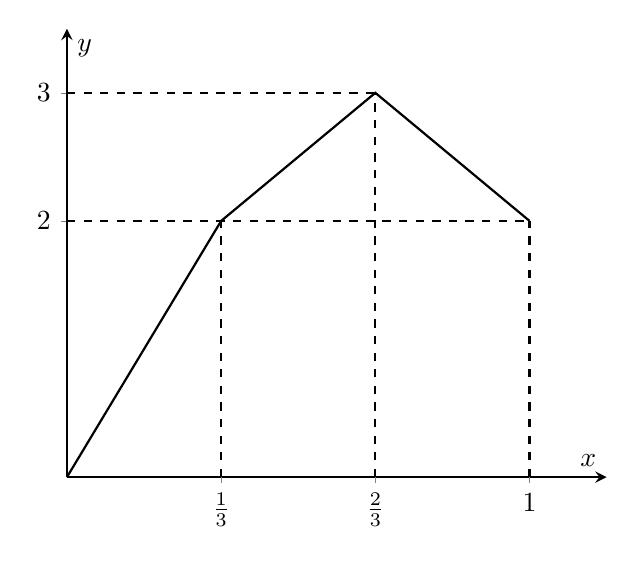
\begin{tikzpicture}
      \begin{axis}[
          axis lines=middle, 
          xticklabels={},
          xtick={1,...,3},
          ytick={2,...,3},
          extra x ticks={1,2,3},
          extra x tick labels={$\frac{1}{3}$,$\frac{2}{3}$,$1$},
          xmin=0, xmax=3.5,
          ymin=0, ymax=3.5,
          xlabel={$x$}, ylabel={$y$},
          samples=200,
          %domain=0:1,
          thick
      ]
      \addplot[no marks] table {
        x   y
        0   0
        1   2
        2   3
        3   2
        };
      \addplot[no marks,dashed] table {
        x y
        0 2
        3 2
        };
      \addplot[no marks,dashed] table {
        x y
        0 3
        2 3
        };
      \addplot[no marks,dashed] table {
        x y
        1 0
        1 2
        };
      \addplot[no marks,dashed] table {
        x y
        2 0
        2 3
        };
      \addplot[no marks,dashed] table {
        x y
        3 0
        3 2
        };
    \end{axis}
  \end{tikzpicture}
\end{figure}
